\chapter{Einleitung}\label{chapter:Einleitun}
Im Folgenden wird für die vorliegende Arbeit anhand der Problemstellung und der daraus folgenden Zielsetzung der Aufbau und damit das Vorgehen für die nachfolgenden Kapitel erläutert.
\section{Problemstellung und Zielsetzung}\label{section:Problemstellung-und-Zielsetzun}
TEST

\section{Aufbau der Arbeit}\label{section:Aufbau-der-Arbei}

Am Anfang\footcite[Vgl.][1]{vomBrocke.2004}\nzitat\footcite[Vgl.][1]{vomBrocke.2004}

\begin{figure}[H]
\centering
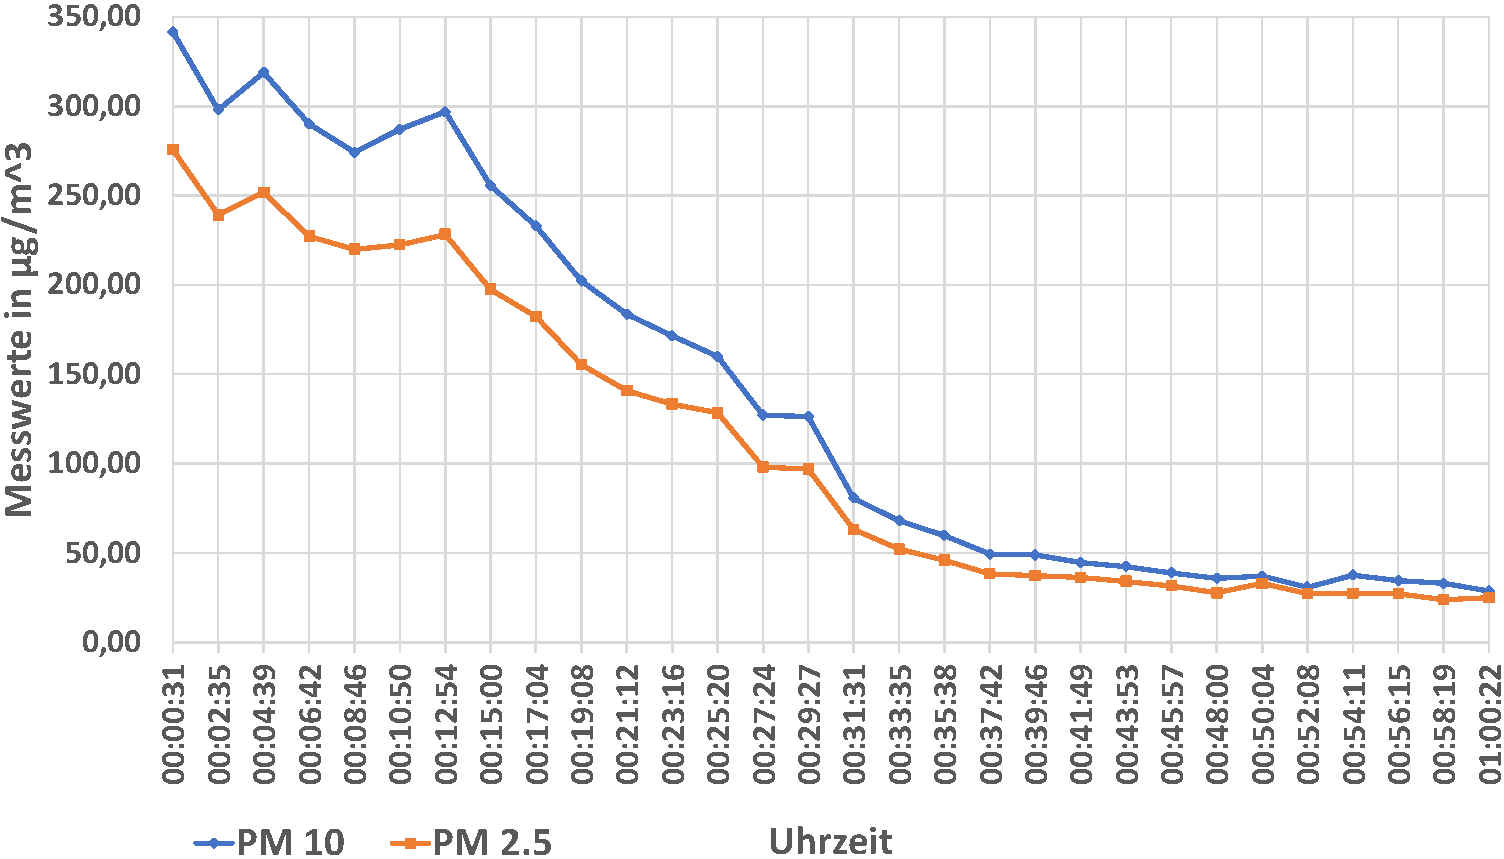
\includegraphics[width=\linewidth]{graphics/Feinstaub-Stuttgart.pdf}
\caption[TEST.]{TEST.\footnotemark}
\label{abb:Grafik}
\end{figure}
\footnotetext{\cite[Entnommen aus:][1]{vomBrocke.2004}}

\begin{table}[H]
\centering
\begin{tabular}{lcr}
links & Mitte & rechts \\
\hline
Muster & Muster & Muster \\
\end{tabular}
\caption{Kleine Beispiel-Tabelle.}
\label{tab:BeispielTabelleKlein}
\end{table}

\TodoW{Write Einleitung}

\ac{LoRaWAN}

\begin{listing}[H]
\inputminted[frame=lines,breaklines=true]{bash}{update_files.sh}
\caption[Skript]{Skript\footnotemark}
\label{listing:percentiles-elasticsearch}
\end{listing}
\footnotetext{\cite[Mit Änderungen entnommen aus][1]{vomBrocke.2004}}